\documentclass[10pt]{beamer}

\usepackage{../macros}
\title{Les séquences : listes}

\hypersetup{
  pdftitle =  {Les séquences : listes}
}

\begin{document}

\maketitle

%%%%%%%%%%%%%%%%%%%%%%%%%%%%%%%%%%%%%%%%%%%%%%%%%%%%%%%
%%%%%%%%%%%%%%%%%%%%%%%%%%%%%%%%%%%%%%%%%%%%%%%%%%%%%%%
%%%%%%%%%%%%%%%%%%%%%%%%%%%%%%%%%%%%%%%%%%%%%%%%%%%%%%%
\begin{frame}[fragile]
  \frametitle{Qu'est-ce qu'une séquence ?}

  \begin{alertblock}{Séquence}
    Une séquence est une suite finie de valeurs numérotées, distinctes ou pas, de n'importe quel type.   
  \end{alertblock}

 
\begin{columns}[t]
\begin{column}{0.48\textwidth}
 \begin{block}{Vecteur}
    Un vecteur est une séquence d'éléments \alert{du même type}.
    \begin{lstlisting}
 > 1:6
[1] 1 2 3 4 5 6
> c('foo', 'bar')
[1] "foo" "bar"     
    \end{lstlisting}
  \end{block}
\end{column}
\begin{column}{0.48\textwidth}
   \begin{block}{Liste}
     Une liste est une séquence d'éléments \alert{de type quelconque}.
     \begin{lstlisting}
> list(1:6, c('foo', 'bar'))
[[1]]
[1] 1 2 3 4 5 6

[[2]]
[1] "foo" "bar"       
     \end{lstlisting}
  \end{block}
\end{column}
\end{columns}

  \begin{block}{Mutabilité}
    Les listes et vecteurs sont mutables, i.e. on peut les modifier.    
  \end{block}
\end{frame}


%%%%%%%%%%%%%%%%%%%%%%%%%%%%%%%%%%%%%%%%%%%%%%%%%%%%%%%
\begin{frame}[fragile]
  \frametitle{De l’utilité des listes \dots}
  
  \begin{exampleblock}{Comment représenter $n$ points de $\mathbb{R}^2$ ?}
    On numérote les points qui appartiendront en fait à $\mathbb{F}^2$. 
  \end{exampleblock}

 \begin{block}{Liste avec 2 vecteurs de taille $n$ (Version I)}
      \begin{itemize}
      \item Le vecteur \texttt{x} contient les abscisses points.
      \item Le vecteur \texttt{y} contient les ordonnées des points.
      \end{itemize}
 \end{block}

  \begin{exampleblock}{Un carré tourné à 45 degrés}
   \begin{lstlisting}[style=block]
> li <- list(c(-1, 0, 1, 0), c(0, -1, 0, 1)) 
   \end{lstlisting}   
 \end{exampleblock}

 \begin{block}{Liste de $n$ vecteurs de taille 2 (Version II)}
   Chaque vecteur contient l'abscisse et l'ordonnée d'un point.
 \end{block}

  \begin{exampleblock}{Un carré tourné à 45 degrés}
   \begin{lstlisting}[style=block]
> li <- list(c(-1, 0), c(0, -1), c(1, 0), c(0, 1)) 
   \end{lstlisting}   
 \end{exampleblock}


 
  \begin{alertblock}{Les listes sont partout !}
    Les structures de données à plusieurs dimensions sont souvent des listes décorées.
  \end{alertblock}
    
\end{frame}


%%%%%%%%%%%%%%%%%%%%%%%%%%%%%%%%%%%%%%%%%%%%%%%%%%%%%%%
\begin{frame}[fragile]
  \frametitle{Accès par rang aux éléments d'une liste}
  \begin{alertblock}{Attention aux différences entre vecteurs et listes }
  \begin{itemize}
  \item La notation indexée par \alert{double crochets}. 
  \item Les indices commencent à 1.
  \item R renvoie une erreur quand les indices sont négatifs.
  \item L'accès par rang devient différent de l'extraction par tranches.
  \end{itemize}
  \end{alertblock}
  
  \begin{lstlisting}
> li <- list(c(-1, 0), c(0, -1), c(1, 0), c(0, 1)) 
> li[[2]] # renvoie un vecteur !
[1]  0 -1
> li[[-2]] 
Error in li[[-2]] : 
  attempt to select more than one element in get1index <real>
> li[[2:3]] 
Error in li[[2:3]] : indice hors limites
\end{lstlisting}
\end{frame}


%%%%%%%%%%%%%%%%%%%%%%%%%%%%%%%%%%%%%%%%%%%%%%%%%%%%%%%
\begin{frame}[fragile]
  \frametitle{Construction d'une nouvelle liste}
  \begin{alertblock}{Construction en extension}
    On utilise surtout la fonction \alert{\texttt{list}}.
    \begin{lstlisting}
> li <- list(42, "foo", TRUE, 1:10)
\end{lstlisting}
  \end{alertblock}

  \begin{block}{Concaténation de deux séquences}
    On peut coller côte à côte (concaténer) deux séquences.
    \begin{lstlisting}
> li1 <- list(42)
> li2 <- list("foo")
\end{lstlisting}
\end{block}    

\vspace{-15pt}
\begin{columns}[t]
  \begin{column}{0.48\textwidth}
    \begin{block}{Concaténation}
    \begin{lstlisting}[style=block]
> append(li1, li2) 
[[1]]
[1] 42

[[2]]
[1] "foo"
\end{lstlisting}
\end{block}

\end{column}
\begin{column}{0.48\textwidth}
  \begin{block}{Création d'une liste de listes}
    \begin{lstlisting}[style=block]
> list(li1, li2) # création d'une liste de listes 
[[1]]
[[1]][[1]]
[1] 42

[[2]]
[[2]][[1]]
[1] "foo"
\end{lstlisting}
  \end{block}
\end{column}
\end{columns}


\end{frame}
%%%%%%%%%%%%%%%%%%%%%%%%%%%%%%%%%%%%%%%%%%%%%%%%%%%%%%%
\begin{frame}[fragile]
  \frametitle{Extraction d'une tranche d'une liste}
  La notation des tranches (\alert{slices}) est valide pour toute séquence. \\
  \begin{itemize}
  \item Comme pour les vecteurs, on utilise les \alert{crochets simples}.
  \item Le résultat est une liste.
  \end{itemize}

    \begin{lstlisting}
> li <- list(c(-1, 0), c(0, -1), c(1, 0), c(0, 1)) 
\end{lstlisting}    

\vspace{-15pt}
\begin{columns}[t]
\begin{column}{0.48\textwidth}
  \begin{exampleblock}{Vecteur numérique d’indices}
    Avec duplication.
    \begin{lstlisting}
> li[c(1,3,3)]
[[1]]
[1] -1  0

[[2]]
[1] 1 0

[[3]]
[1] 1 0
\end{lstlisting}    
  \end{exampleblock}
\end{column}
\begin{column}{0.48\textwidth}
  \begin{exampleblock}{Vecteur logique d’indices}
    Avec recyclage.
    \begin{lstlisting}
> li[c(TRUE, FALSE)]
[[1]]
[1] -1  0

[[2]]
[1] 1 0
\end{lstlisting}    
  \end{exampleblock}

\end{column}
\end{columns}
Comme pour les vecteurs, on peut utiliser les fonctions d'extraction \texttt{head} et \texttt{tail}.


\end{frame}

%%%%%%%%%%%%%%%%%%%%%%%%%%%%%%%%%%%%%%%%%%%%%%%%%%%%%%%
\begin{frame}[fragile]
  \frametitle{Autres opérations sur les listes}
  
  \begin{block}{Modification d'une liste}
    Avec l'opérateur crochet, la méthode \texttt{append} ou les indices négatifs.
  \begin{lstlisting}[style=block]
> li <- list(c(-1, 0), c(0, -1), c(1, 0), c(0, 1)) 
> li[c(-1, -3, -4)] # suppression d'éléments
[[1]]
[1]  0 -1
\end{lstlisting}  
\end{block}


  \begin{block}{Arithmétique, conditions et tests vectorisés ? }
    Non, on procédera d'autres manières, par exemple par itérations.
    \begin{lstlisting}
> li + li
Error in li + li : argument non numérique pour un opérateur binaire    
> li == li 
Error in li == li : comparaison de ces types non implémentée
> li & li
Error in li & li : 
  ces opérations ne sont possibles que pour des types numériques, logiques ou complexes
\end{lstlisting}

\end{block}

\end{frame}



%%%%%%%%%%%%%%%%%%%%%%%%%%%%%%%%%%%%%%%%%%%%%%%%%%%%%%%
\begin{frame}[fragile]
  \frametitle{Boîte englobante pour un nuage de points}
    \begin{block}{Comment représenter $n$ points de $\mathbb{R}^2$ ?}
      On numérote les points qui appartiendront en fait à $\mathbb{F}^2$.
      \begin{enumerate}
    \item Liste avec 2 vecteurs de taille $n$. 
      \begin{itemize}
      \item Le vecteur \texttt{x} contient les abscisses points.
      \item Le vecteur \texttt{y} contient les ordonnées des points.
      \end{itemize}
    \item Liste de taille $n$ dont chaque élément est un vecteur de taille 2.
      \begin{itemize}
      \item Chaque vecteur contient l'abscisse et l'ordonnée d'un point.
      \end{itemize}
    \end{enumerate}
  \end{block}

  \begin{figure}[htbp]
    \centering
    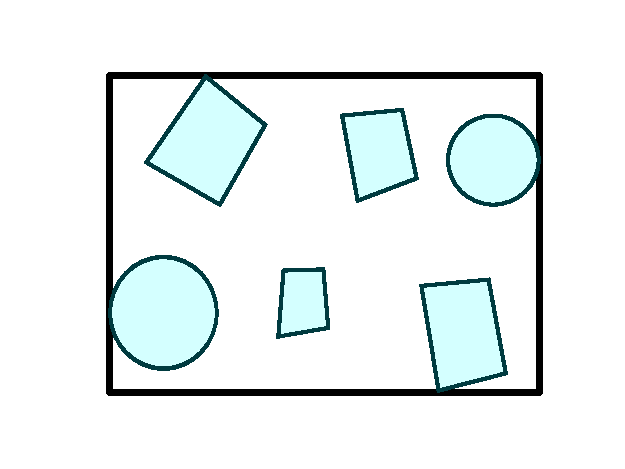
\includegraphics[width=0.4\textwidth]{minimum_bounding_rectangle}
    \caption{Qu'est-ce qu'une boîte englobante ? Merci \href{https://en.wikipedia.org/wiki/Minimum_bounding_box}{Wikipedia}.}
  \end{figure}
\end{frame}

%%%%%%%%%%%%%%%%%%%%%%%%%%%%%%%%%%%%%%%%%%%%%%%%%%%%%%%
\begin{frame}[fragile]
  \frametitle{Boîte englobante (Version I)}
  

  \begin{lstlisting}[style=editor]
CalculerBoiteEnglobante <- function(pts) {
  ## pts est une liste avec 2 vecteurs
  return(list(
   range(pts[[1]]),
   range(pts[[2]])
   ))
}
  \end{lstlisting}


  \begin{lstlisting}
> pts <- list(c(-1, 0, 1, 0), c(0, -1, 0, 1))
> CalculerBoiteEnglobante(pts)
[[1]]
[1] -1  1

[[2]]
[1] -1  1
  \end{lstlisting}

\end{frame}


%%%%%%%%%%%%%%%%%%%%%%%%%%%%%%%%%%%%%%%%%%%%%%%%%%%%%%%
\begin{frame}[fragile]
  \frametitle{Boîte englobante (Version II)}
  

  \begin{lstlisting}[style=editor]
CalculerBoiteEnglobante <- function(pts) {
  ## pts est une liste de n vecteurs
  CalculerIntervalleEnglobant <- function(pts, d) {
    ## on reprogramme la fonction range ...
    a <- Inf
    b <- -Inf
    for(p in pts) {
      if(p[d] < a) a <- p[d]
      if(p[d] > b) b <- p[d]
    }
    return(c(a,b))
  }
  x <- CalculerIntervalleEnglobant(pts, 1)
  y <- CalculerIntervalleEnglobant(pts, 2)
  ## on met en forme le résultat
  return(list(
   c(x[1], y[1]),
   c(x[2], y[2])
   ))
}
  \end{lstlisting}
%   \begin{lstlisting}
% > pts <- list(c(-1, 0), c(0, -1), c(1, 0), c(0, 1)) 
% > CalculerBoiteEnglobante(pts)
% [[1]]
% [1] -1 -1

% [[2]]
% [1] 1 1
% \end{lstlisting}

\end{frame}


%%%%%%%%%%%%%%%%%%%%%%%%%%%%%%%%%%%%%%%%%%%%%%%%%%%%%%%
\questionSlide

%%%%%%%%%%%%%%%%%%%%%%%%%%%%%%%%%%%%%%%%%%%%%%%%%%%%%%%
 \appendix
 \backupSlides
%%%%%%%%%%%%%%%%%%%%%%%%%%%%%%%%%%%%%%%%%%%%%%%%%%%%%%%

%%%%%%%%%%%%%%%%%%%%%%%%%%%%%%%%%%%%%%%%%%%%%%%%%%%%%%%
% \begin{frame}[fragile]{Backup slides}
%   Sometimes, it is useful to add slides at the end of your presentation to
%   refer to during audience questions.

%   The best way to do this is to include the \verb|appendixnumberbeamer|
%   package in your preamble and call \verb|\appendix| before your backup slides.

%   will automatically turn off slide numbering and progress bars for
%   slides in the appendix.
% \end{frame}


%%%%%%%%%%%%%%%%%%%%%%%%%%%%%%%%%%%%%%%%%%%%%%%%%%%%%%%
% \begin{frame}[allowframebreaks]{References}

%   % \bibliography{../bib_parallelism,../bib_others}
%   % \bibliographystyle{abbrv}

% \end{frame}

\end{document}

%%% Local Variables:
%%% mode: latex
%%% TeX-master: t
%%% End:
